\documentclass[conference,compsoc]{IEEEtran/IEEEtran}
% Some/most Computer Society conferences require the compsoc mode option,
% but others may want the standard conference format.
%
% If IEEEtran.cls has not been installed into the LaTeX system files,
% manually specify the path to it like:
% \documentclass[conference,compsoc]{../sty/IEEEtran}


%\documentclass{article}

\sloppy
\usepackage{geometry}
\geometry{letterpaper, margin=1in}
\usepackage[utf8]{inputenc}
\usepackage{graphicx}
%\usepackage[breaklinks=true]{hyperref}
\usepackage{hyperref}
\usepackage[T1]{fontenc}
\usepackage{epstopdf}
\title{\bf Final Project Proposal}
\author{ECE 1373 Winter 2016}
\date{\today}

\begin{document}

\maketitle

\section{Group Members}
Roberto DiCecco, Muhammad Talha Malik, John Adler

\section{Introduction}\label{section:intro}

Convolutional networks are one of the most widely employed architectures in machine learning. Although convolutional networks deliver impressive results across a range of machine learning tasks, they are computationally demanding which limits their deployability. The focus of this project is speeding up the application of convolutional neural networks. Convolutional layers generally consume the bulk of the processing time, and so in this work we present different engines to be used for speeding up these layers.

Our group will be performing an architecture exploration of the convolution layers commonly found in 
Convolutional Neural Networks (CNNs). The architectures we will be exploring will be based off of three
different approaches for implementing convolutions: the nested-loop based approach to convolutions, 
the matrix multiply based approach, and the Fast Fourier Transform (FFT) based approach. The architecture
exploration will target multiple sizes of convolutional layers, with the network in question being AlexNet. 

One of the simplest approaches to implementing convolution is to implement it without any pre-processing of the data.
This can be done by implementing convolution based off of equation \ref{eq:conv} as a series of nested loops. This has been
the focus of other works, namely \cite{conv_zhang} which achieved significantly higher performance than prior implementations. 
This approach has the potential for high levels of parallelism as the multiplications and many of the accumulations can be done
in parallel. 

\begin{equation}\label{eq:conv}
C_{i,j} = \sum_{p=0,q=0}^{p=K_x,q=K_y}A_{i\cdot S_y + p, j\cdot S_x + q}\cdot B_{p,q} 
\end{equation}
Where\\ 
\hspace*{2em} $C_{i,j}$ is the output at indices i,j;\\
\hspace*{2em} $K_x$ is the horizontal dimension of the kernel;\\
\hspace*{2em} $K_y$ is the vertical dimension of the kernel;\\
\hspace*{2em} $S_x$ is the horizontal stride;\\
\hspace*{2em} $S_y$ is the vertical stride;\\
\hspace*{2em} A is the input frame;\\
\hspace*{2em} B is the kernel frame.\\

An alternative approach to performing the calculations involves using matrix multiplication.
The key to this approach is that the convolution operation is essential a series of dot products.
To take advantage of this, data is first preprocessed by ``stretching'' it -- replicating values into a larger matrix in a specific order, dependent on the filter dimensions.
This new matrix can then be sent directly to one of many efficient linear algebra solvers, such as BLAS (which is used in the Caffe framework).
The resultant matrix is the compressed back to the desired output dimensions of the convolutional layer.

Fourier transforms can provide a significant speedup in the computation of convolutions in CNNs \cite{FFT1, FFT2}. This computational gain arises from the convenient property of operator duality between convolution in the spatial domain and element-wise multiplication in the frequency domain. In this project, we will use the Fast Fourier Transform (FFT) algorithm to accelerate the training and inference in CNNs.


\section{Goal}\label{section:goal}

The goal of this project is to evaluate the performance -- runtime and area in this case, since performance in a machine learning context usually means accuracy -- of various hardware implemententions of convolutional layers.
Using the three techniques outlined in Section~\ref{section:intro}, optimized hardware implementations that will run on an FPGA will be designed.
These will then be benchmarked against existing CPU and GPU implementations, with the expectation that (some of) the new hardware implementations will be able to achieve improved performance.

\section{Specifications}\label{section:spec}

\begin{itemize}
\item The board that we will be using is the ADM-PCIE-7V3 Xilinx Alpha Data card
with Virtex-7 690T. The reason for this selection is to take advantage of the
Xilinx SDAccel platform for the project.

\item The system will involve several different engines to be used for computing
convolution for Convolutional Neural Networks (CNNs). Each convolution engine
will be implemented as one of three different potential architectures: a direct
convolution engine, a matrix multiply based convolution engine, and a Fast Fourier
Transform based convolution engine.

\item The final system will be able to classify images using the AlexNet CNN, with 
comparable accuracy to the baseline implementations found in Caffe. 

\item Peripheral Requirements: no other equipment is required other than the machine
containing the ADM-PCIE-7V3.

\item Constraints and limitations: the designs are required to operate at 200MHz due
to the board specifications and they must be written in C or OpenCL and be compatible
with the Xilinx SDAccel platform.
\end{itemize}

\section{System Overview}\label{section:overview}

The high-level synthesis flow that will be used for this project will be the Xilinx 
SDAccel flow. This will be used to implement each potential architecture for the 
AlexNet convolutional layers. 

The system that we will build for this project is the AlexNet CNN, though the work 
will be applicable to other CNNs as well. The design of this system will involve the 
selection between several different algorithms for the convolutional layers of the 
network as outlined in \ref{section:intro}. These implementations will then be ported
to the Caffe CNN framework to be used within a full CNN (AlexNet). 

Each convolutional layer will be designed with two potential constraints in mind: 
maximum throughput for a given layer without area constraints and maximum throughput
for a given layer with area constraints to allow for the accommodation of other 
layers. The other layers in question are the ReLU, LRN, Pooling, and Fully Connected
layers which have already been implemented. 

\subsection{Matrix Multiplication Algorithm}
Implementing a matrix multiplication algorithm efficiently in hardware similar to that implemented in software in the Caffe framework will be challenging.
Replicating data for the purpose of parallelizing computations is a straightforward task in software, but cannot be done in hardware without severe performance penalties due to the tight area constraits of an FPGA board.
To work around this constraint, the control logic of accessing matrix elements can be parallelized instead.~\cite{MM_strassen,MM_efficient}

\subsection{FFT-based Algorithm}
Convolutional layers generally consume the bulk of the processing time in CNNs. In order to reduce this time, we will implement an algorithm that computes convolutions as element wise multiplication in the Fourier domain. Not only this requires significantly less operations to compute, but it also exposes extra level of parallelism which is a very desirable characteristic in FPGAs. An FFT-based convolution for each convolutional layer can be broken up into $3$ steps as shown in Fig.~\ref{CNN-FFT}: an FFT of the input images and the filters, elementwise products followed by a sum across input channels, and then an inverse FFT (iFFT) of the outputs.

Although convolutions can be computed efficiently as products in the Fourier domain, the overheads incurred in computing the FFTs and iFFTs can be significant depending on the size of the inputs and filters. Modern convolutional networks use large size filters which makes the overheads of computing the FFTs worthwhile because we can effectively reuse our FFTs many times which compensates for the overhead \cite{FFT1}.

There are some potential drawbacks associated with this approach. Computing direct convolution is much easier to implement in practice as compared to a well tuned FFT implementation. In addition to its complexity, the FFT requires feature maps to be padded to a special size, such as a power of two. Moreover, additional memory is required to store the filter matrices in the Fourier domain which might become prohibitively expensive in terms of memory for large networks.

\subsection{Direct Convolution} 
Implementing convolution using Equation \ref{eq:conv} could present challenges with respect to standard CPU or GPU architectures
due to the amount of branching required along with the strided access patterns. In the case of FPGAs, we can customize the hardware 
to suit the access and branching patterns of the system, such that there is negligible performance loss while achieving high
levels of parallelism with this approach. High-level synthesis directives allow for the parallelism of the algorithm to be better
exploited through the use of unroll and pipeline directives as needed. 

This approach can potentially result in high performance for certain convolution layers as there is minimal pre-processing overhead
required prior to computing the results. On the other hand, it may be much more difficult to achieve higher performance in the case of
larger filter sizes as the area and timing requirements to unroll these sorts of layers may be prohibitively expensive. 

\begin{figure}[!h]
\begin{center}
\centering
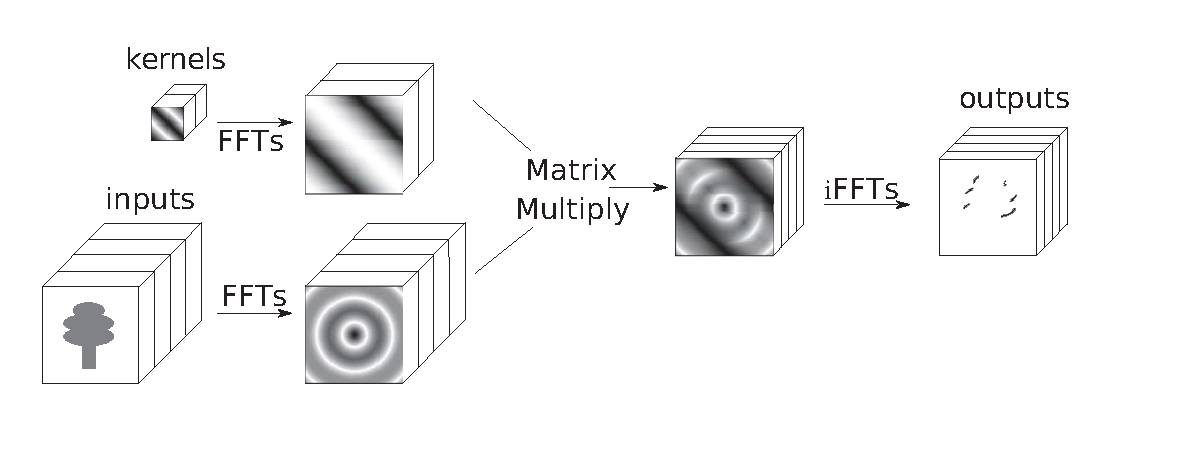
\includegraphics[width=1\columnwidth]{CNN-FFT.eps}
\caption{Block diagram showing FFT-based convolution in CNNs}
\label{CNN-FFT}
\end{center}
\end{figure}

\section{Testing}\label{section:testing}

The testing procedure will be segmented into three primary steps for each design in the project.
The first step will involve algorithmic testing in a separate C testbench similar to the usual C
simulation in Vivado HLS. This process will be conducted while experimenting with the algorithms
to improve throughput. The second step will involve using test benches within the Caffe environment
to ensure that the HLS kernels are properly integrated with the Caffe source code. Finally, the
hardware versions of the HLS kernels will be tested within the framework using the Alexnet network
against a subset of the Imagenet validation set to ensure functional correctness and accuracy
within the full system.

\section{Risk}\label{section:risk}

One primary risk for the project is that ramp up time for the toolset could be longer than 
anticipated, which could result in delays with respect to finishing the design of each kernel. 
To try to mitigate this risk factor, we will plan to coordinate an initial task devoted to
learning how to use SDAccel. 

The strengths of our team are that we all have familiarity with machine learning algorithms,
with Roberto and John both having experience with the Caffe CNN framework as well. One of the 
main weaknesses of the team is that for the most part the tools will be relatively new to use,
so tool related issues could be a problem in the future. 

\section{Milestones}\label{section:milestones}

\begin{itemize}
    \item The first week will involve a ramp-up exercise to familiarize Muhammad and John with 
	the SDAccel tools through a simple HLS kernel (e.g. "Hello World"). 
    \item Also in the first week, Roberto will implement a reprogram layer inside of Caffe to 
	allow for the reprogramming of the FPGA to be decoupled from the kernel execution 
	(this functionality has been implemented, but needs to be refined through a separate layer). 
    \item In the second week, each of us will create our C implementations of the algorithms 
	that we are each targeting for each of the convolution layers. Roberto: Direct convolution 
	using nested loops, Muhammad: FFT based convolution, John: matrix multiply based convolution. 
	\item In the second week, Roberto will also make some updates to the framework to accommodate
	multiple layers in a single binary, and update it to include batch support. 
    \item In the following two weeks each of us will focus on trying to improve throughput of our 
	respective designs under the different layer constraints of AlexNet.
    \item Afterwards, we will analyze the results of the respective designs, and decide which 
	architecture will be suitable for the respective layers. Then we will begin system integration 
	with Caffe.
    \item In the last week we will conduct additional tests of the system with images from the 
	ImageNet validation database. 
\end{itemize}


\bibliographystyle{IEEEtran}
\bibliography{references}

\end{document}
